%

\section{Dataset} \label{sectionDataset}
To evaluate HMOG features, we used sensor data collected from 100 smartphone users (53 male, 47 female) during eight free text typing sessions~\cite{qingPoster}.\footnote{Our dataset is available at \url{ http://www.cs.wm.edu/~qyang/hmog.html}} Users answered three questions per session, typing at least 250 characters for each answer. In four sessions, the users typed while sitting. In another four sessions, users typed while walking in a controlled environment.

For each user, we collected an average of 1193 taps per session (standard deviation: 303) and 1019 key presses (standard deviation: 258). The average duration of a session was 11.6 minutes, with a standard deviation of 4.6 minutes.
Data was collected using the same smartphone model (Samsung Galaxy S4). We used a total of ten Samsung Galaxy S4. Data was collected over multiple days, and the same user might have received a different device during each visit.

%
%
%
%
%
%
%
%
%
%
%
%
%
%
%
%
%
%
%

We recorded accelerometer, gyroscope and magnetometer sensor readings (sampling 
rate 100~Hz) as well as raw touch data collected from the touchscreen, touch 
gestures (e.g., tap, scale, scroll, and fling), key press, and key release 
latencies on the virtual keyboard. Due to security concerns, Android OS forbids 
third-party applications to access touch and key press data generated on the 
virtual keyboard. Therefore, we designed a virtual keyboard for data collection 
that mimicked the look, feel, and functionality of default Android keyboard, 
including the autocorrect and autocomplete options, which the users were free to use.

During data collection users were allowed to choose the orientation of the 
smartphone (i.e., landscape or portrait). Because less than 20 users typed in landscape orientation, we performed all authentication experiments with data collected in portrait mode.



\section{Evaluation of HMOG Features} \label{sectionExperiments} 


%

\begin{figure}[htbp]
   \centering
   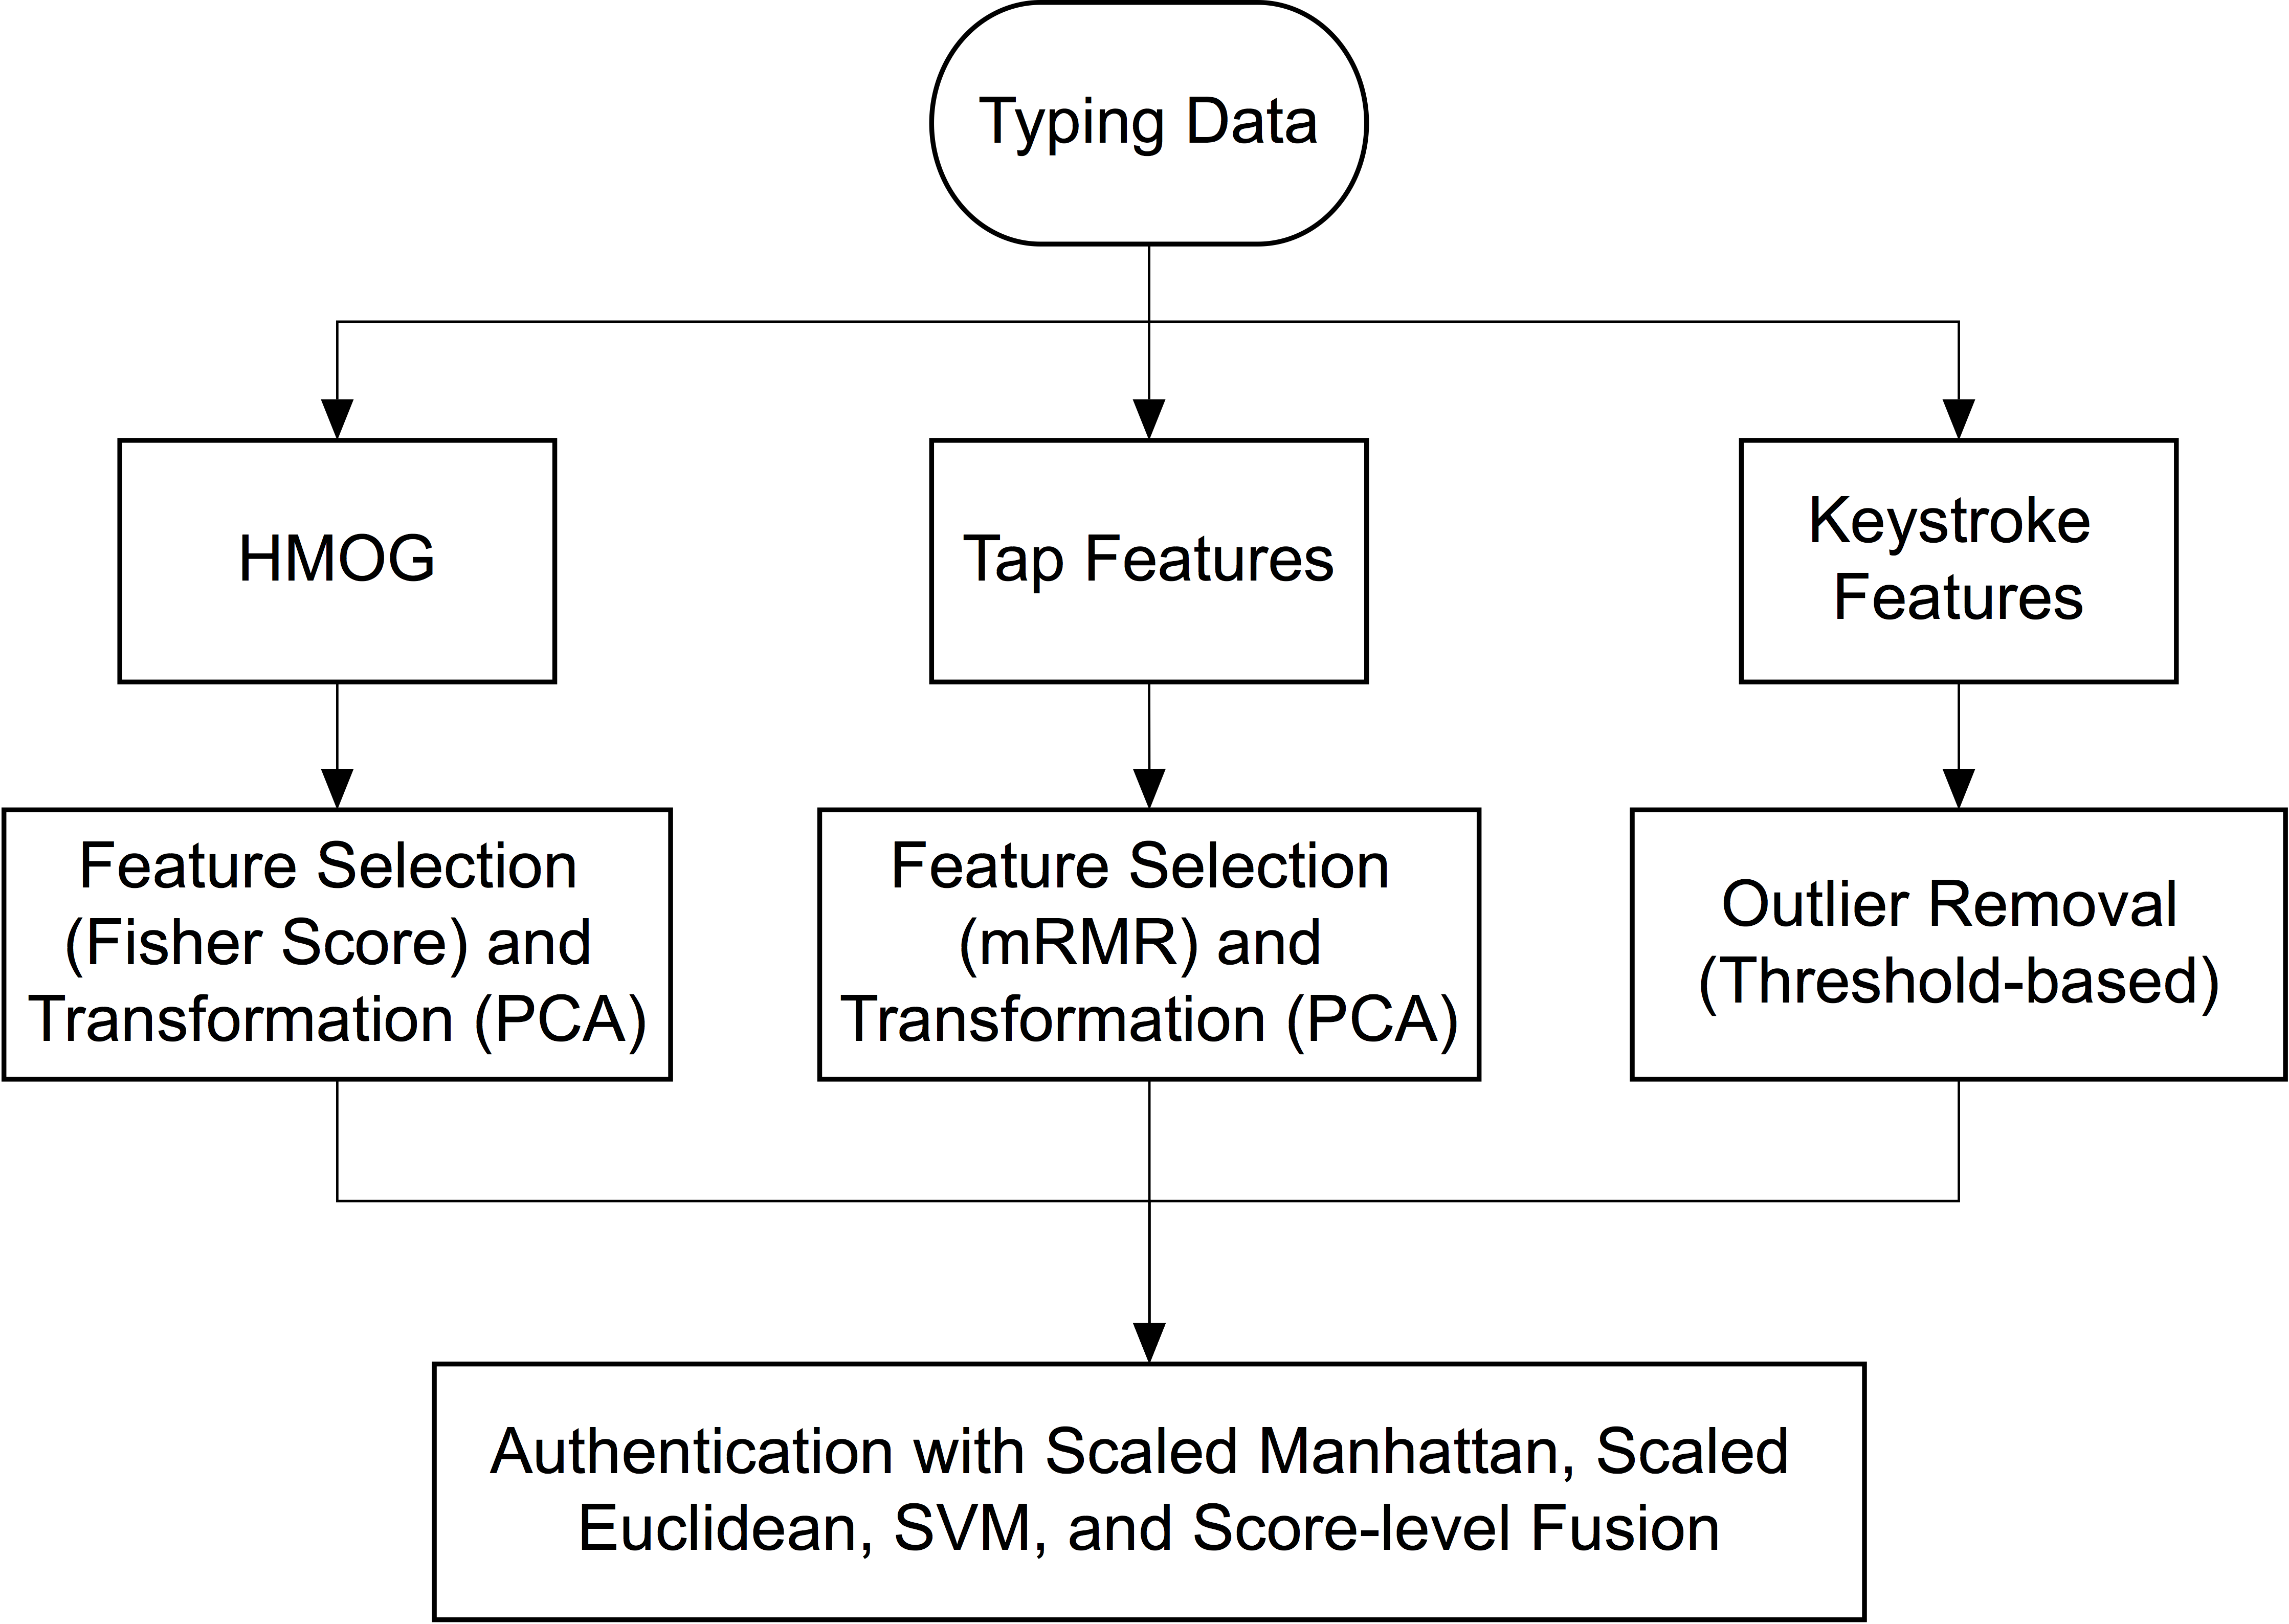
\includegraphics[width=0.8\linewidth]{FlowChartHMOG.png} %
   \caption{Flow-diagram depicting our experiment workflow.}
   \label{fig:flowchart}
\end{figure}

Our experiment workflow involves: (1) computing features from data collected during typing; (2) performing feature selection; (3) performing feature transformation (PCA); (4) performing  outlier removal; and (5) performing authentication using  Scaled Manhattan, Scaled Euclidean, SVM verifiers, and score-level fusion. 
Figure~\ref{fig:flowchart} summarizes the experiment workflow.


\subsection{Design of Authentication Experiments} \label{authenticationExperiments}

 
\paragraph{1-Class Verifiers} We performed verification experiments using three verifiers~\cite{maxion2009}: scaled Manhattan (SM), scaled Euclidian (SE), and 1-class SVM. (Henceforth, we use ``SVM'' to refer to ``1-class SVM''.) We chose these verifiers because previous work on behavioral authentication has shown that they perform well. For instance, SM and SVM were top performers in a study on keystroke authentication of desktop users by Maxion et al.~\cite{maxion2009}. SVM performed well in experiments on touch-based authentication of smartphone users by Serwadda et al.~\cite{serwadda2013}. SE is a popular verifier in biometrics (see for example~\cite{blanton2011,govindarajan2013}). 
 
 
Parameter tuning was not required for SM and SE. However, for SVM~\cite{libSVM}, we used RBF kernel and performed a grid search to find the parameters (for $\gamma$, we searched through $2^{-13}$, $2^{-11}$,  $2^{-9}$, \dots, $2^{13}$; and for $\nu$, we searched through 0.01, 0.03, 0.05, 0.1, 0.15 and 0.5). We used cross-validation to choose the parameter values (see Section~\ref{featurePreparation}).
 
We did not include 2-class verifiers in our evaluation. To train a 2-class verifier, in addition to data from smartphone owner, biometric data from other users (non-owners) is required. Because sharing of biometric information between smartphone users leads to privacy concerns, we believe that 1-class verifiers are more suitable for smartphone authentication. (A similar argument was made in~\cite{shen2013user}.)


\paragraph{Training and Testing}  For experiments in sitting and walking conditions, we used the first two sessions for training and the remaining two for testing. We extracted HMOG features during each tap. Thus, each training/testing vector corresponded to one tap. With keystroke dynamics features, each training/testing vector corresponded to one key press on the virtual keyboard.%

For SM and SE, the template consisted of the feature-wise average of all training vectors. We used user-wise standard deviations for each feature for scaling. We used all training vectors to construct the template (hypersphere) with SVM.
%
%
Users with less than 80 training vectors were discarded from authentication. As a consequence, ten users failed to enroll (and were not included in our experiments). 


We created authentication vectors by averaging test vectors sampled during $t$-seconds scan. We report results for authentication scans of $t$ = 20, 40, 60, 80, 100, 120 and 140 seconds. We chose these scan lengths to cover both low and higher authentication latencies. Our preliminary experiments showed that for scans longer than 140 seconds, there is minimal improvement in authentication performance. 

\paragraph{Quantifying Authentication Performance}
We generated two types of scores, genuine (authentication vector was matched against template of the same user) and zero-effort impostor (authentication vector of one user was matched against the template of another). We used population equal error rate (EER) to measure the authentication performance.


\subsection{Comparing HMOG to Other Feature Sets}
We compared the authentication performance of HMOG features with touchscreen tap and keystroke dynamic features (key hold and digraph latencies). 

%


\paragraph{Touchscreen Features from Tap Events} 
We extracted 11 commonly used touchscreen-based features for tap events (see~Table \ref{tab:relatedResearch}). Some papers (e.g.,  \cite{serwadda2013} and \cite{frank2013}) defined these features for swipes, while we extracted them from {\em taps} due to very low availability of swipes during typing, and to provide a more meaningful comparison with HMOG features, which are collected during taps. The features we extracted are: 
\begin{itemize}
\item Duration of the tap
\item Contact size features: mean, median, standard deviation, 1st, 2nd and 3rd quartile, first contact size of a tap, minimum and maximum of the contact size during the tap (9 features) 
\item Velocity (in pixels per second) between two consecutive \textit{press} events belonging to two consecutive taps.
\end{itemize}


\paragraph{Key Hold Features}
Key hold latency is the down-up time between press and release of a key. We used 89 key hold features, each corresponding to a key on the virtual keyboard. 

\paragraph{Digraph Features}
Digraph latency is the down-down time between two consecutive key presses. We used digraph features for combinations of the 35 most common keys in our dataset.\footnote{All 26 alphabetic keys, 5 keyboard switches (shift, switch between numerical and alphabetical keyboard, delete, done, return) and 4 special characters (space, dot, comma and apostrophe). The availability of other keys in our training data was extremely low ($< 1$ on average per user).} Thus we have $35^2 = 1225$ digraph features.%


\paragraph{Score-level Fusion}
To determine whether HMOG features complement existing feature sets, we combined tap, key hold, digraph and HMOG features using weighted sum score-level fusion. We chose this method because it is simple to implement, and has been shown to perform well in biometrics~\cite{ross2003}. We used the technique of Locklear et al.~\cite{locklear2014} to ensure that weights sum to one and proportion of weights is preserved when scores from some feature sets were missing (e.g. due to lack of accelerometer data). We used grid-search to find the weights which led to the best authentication performance.


\subsection{Feature Selection, Preprocessing, and Transformation} \label{featurePreparation}
To improve  authentication performance, we performed feature selection, feature transformation with Principal Component Analysis (PCA), and outlier removal. %
%
%
%
%
%
%


%

\paragraph{Parameter selection}
We used 10-fold cross-validation (10-CV) on training data to choose feature selection method (mRMR or Fisher score ranking), as well as to set the parameters for feature selection, PCA, and SVM. The parameters are presented in Table \ref{cvparams}. We evaluated all parameters independently for each combination of feature set, verifier, authentication scan-length and body-motion condition. 

\begin{table}
\caption{Parameters evaluated using cross-validation} \centering
\begin{tabular}{ l  l  }
\hline
Method & Parameter \\ \hline
Fisher score & Percentage of the sum of all Fisher scores \\
mRMR & Threshold on the mRMR score\\
PCA & Percentage of total variance \\
SVM & $\gamma$, $\nu$ \\
\hline
\end{tabular}
\label{cvparams}
\end{table}



%
For each set of parameter values, 10-CV yielded ten EERs, which we averaged to get an estimate of the EER corresponding to that set of parameter values. We then selected parameter values which had the lowest (average) EER. For 10-CV experiments involving 20- to 140-second scan lengths, the sets of parameter values that led to the lowest EERs were not always identical. In this case, we took a majority vote to select the most common parameter values.

\paragraph{Feature Selection} 
%
During training, we evaluated two feature selection methods: Fisher score ranking~\cite{duda2001pattern}, 
and minimum-Redundancy Maximum-Relevance (mRMR)~\cite{mRMR}. 
Our preliminary experiments showed that Fisher score performed better for HMOG features, while mRMR performed well with tap features. With key hold and digraph features, the best performing feature set contained all the features.

Fisher score ranking 
was computed independently for each HMOG feature as the ratio of {\em between-user} 
to {\em within-user} variance. (Higher Fisher score suggests higher 
discriminability of the corresponding feature.) Using 10-CV, we tested feature 
subsets whose sum of Fisher scores accounted for 80\% to 100\% of the 
sum of Fisher scores of all features.  

We selected HMOG features for each verifier separately. The following parameters 
for Fisher score ranking provided the best authentication results: 82\% (17 features) for SM
during sitting; 81\% (13 features) for SM and SVM during walking; and 80\% (16 features) for SVM during sitting. For SE, we achieved lowest EER by including resistance features only, compared to the feature subset obtained from feature selection. %
%
%
Figure~\ref{fig:fisherFeatures} reports the ranking of the features during sitting (\ref{fig:fisherFeaturesSit}) and walking (\ref{fig:fisherFeaturesWalk}).


\begin{figure}[tb] 
\subfigure[Fisher scores of HMOG features during sitting.]{\label{fig:fisherFeaturesSit}
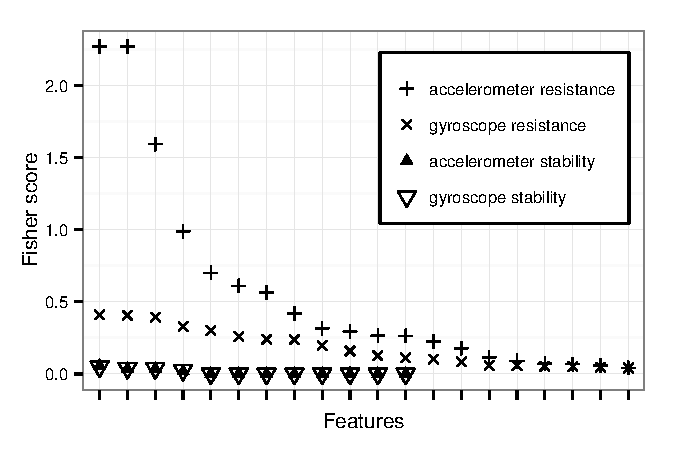
\includegraphics[width=1\linewidth]{plots_R/FisherFeaturesSit.pdf} 
}

\subfigure[Fisher scores of HMOG features during walking.]{\label{fig:fisherFeaturesWalk}
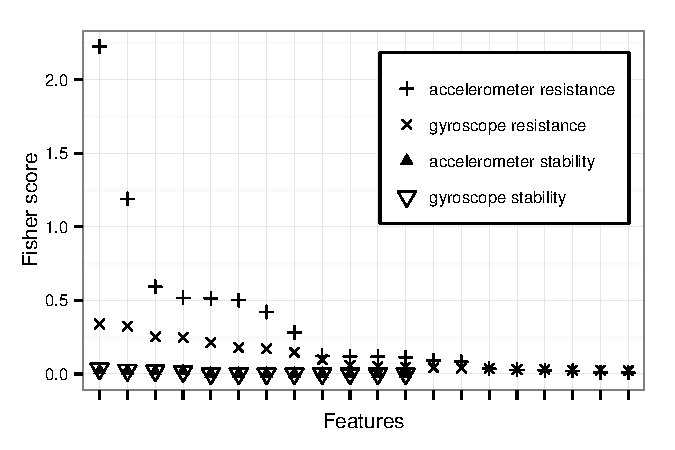
\includegraphics[width=1\linewidth]{plots_R/FisherFeaturesWalk.pdf} 
}

\caption[]{HMOG features extracted from accelerometer and gyroscope, sorted by Fisher score computed from training data. Higher scores correspond to features with higher discriminative power. 
%
Magnetometer features (not shown) ranked below accelerometer and gyroscope features.
}
 \label{fig:fisherFeatures}
\end{figure}

For tap features, with SM verifier we achieved the best results  with 3 features chosen by mRMR (threshold 0) and for SE and SVM with 2 features (threshold 0.1). The best three features according to mRMR are (in this order): duration of the tap; mean of contact size; and velocity between two consecutive down events. 

\paragraph{Outlier Removal}
For HMOG and tap templates, we evaluated the interquartile outlier removal (i.e., different subsets of the values from the first and fourth quartile are removed). Experiments with SM verifier showed that outlier removal does not improve authentication accuracy, so we did not consider it further in our experiments. 
 %


For key hold and digraph latencies, using only outlier removal and not performing feature selection or transformation led to the best results. Outlier removal was done using two parameters: (1) latencies longer than $l$ ms were discarded and (2) if a feature occurs less than $m$ times in a user's template, the feature was discarded). 
The values evaluated for $l$ were 100, 200, 300, 400, 500 and 1000 for key hold and 200, 350, 500, 650 and 800 for digraph.
 For $m$, we experimented with 2, 5, 10, 15, 20, 40 and 60. 
%
The best $l$ value was 200 for key hold, and between 350--500 for digraph; the best $m$ value was between 2--60 for key hold and between 2--5 for digraph.

\paragraph{Feature Transformation} 
We used PCA to transform original features into principal components, that were subsequently used in authentication experiments. Our motivation for using PCA are: (1) to remove correlation between features to meet the assumptions in SE and SM, and (2) to reduce dimensionality by using only those principal components, which explain most of the variance. We performed PCA under two settings: (1) on all features (except magnetometer features, which performed poorly), and  (2) on a subset of features selected using Fisher score and mRMR. We performed 10-CV experiments with components explaining 90\%, 95\%, 98\%, and 100\% of total variance, to set the threshold for dimensionality reduction. PCA improved EER for HMOG features with SE when performed on resistance features, and for SVM during sitting when performed on features selected using Fisher score. %
PCA performed on all tap features improved results with SM and SE. %

%
%
%

%

%

%
%

%

%
%
%
%




%
%



